\begin{exo}{}
	David et Antoine achètent un terrain qui doit être partagé en deux perpendiculairement à la route principale. On désigne par $x$ la distance entre le chemin d'accès et la ligne de partage comme ci-dessous.
	\begin{center}
		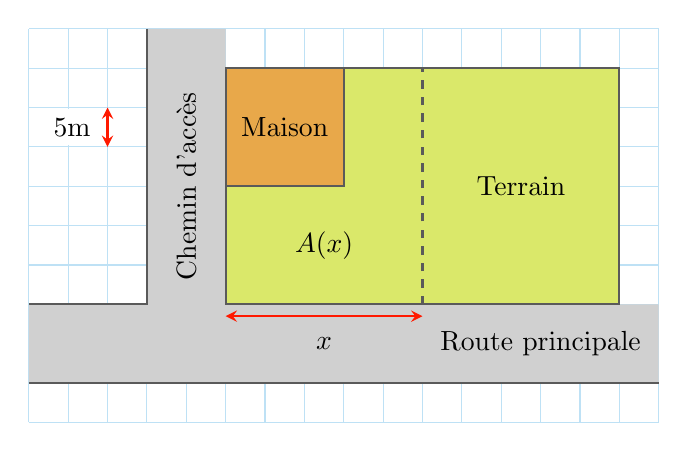
\begin{tikzpicture}[scale=0.5]
			\definecolor{terrain}{RGB}{218,232,106}
			\definecolor{maison}{RGB}{232,168,74}
			\definecolor{route}{RGB}{208,208,208}
			\definecolor{bord}{RGB}{90,90,90}
			\definecolor{grille}{RGB}{190,225,245}
			\draw[grille] (-5,-3) grid (11,7);
			\fill[route] (-2,7) -- (0,7) -- (0,0) -- (11,0) -- (11,-2) -- (-5,-2) -- (-5,0) -- (-2,0) -- cycle;
			\draw[bord, thick] (-2,7) -- (-2,0) -- (-5,0);
			\draw[bord, thick] (-5,-2) -- (11,-2);
			\filldraw[fill=terrain, draw=bord, thick] (0,0) rectangle (10,6);
			\filldraw[fill=maison, draw=bord, thick] (0,3) rectangle (3,6);
			\draw[bord, thick, dashed] (5,0) -- (5,6);
			\draw[red!80!orange, thick, <->, >=stealth] (0,-0.3) -- (5,-0.3);
			\node at (2.5,-1) {$x$};
			\draw[red!80!orange, thick, <->, >=stealth] (-3,4) -- (-3,5);
			\node[fill=white] at (-3.9,4.5) {$5$m};
			\node at (1.5,4.5) {Maison};
			\node at (7.5,3) {Terrain};
			\node at (2.5,1.5) {$A(x)$};
			\node[rotate=90] at (-1,3) {Chemin d'accès};
			\node at (8.0,-1) {Route principale};
		\end{tikzpicture}
	\end{center}

	\textbf{Partie 1 :}
	
	\begin{enumerate}
		\item Déterminer l'ensemble de définition de $x$ et l'aire totale du terrain en jaune sans prendre en compte la maison.
	\end{enumerate}
	
	Soit $A(x)$ l'aire du terrain de gauche longeant le chemin d'accès sans prendre en compte la maison.
	
	\begin{enumerate}[resume]
		\item
		      \begin{enumerate}
			      \item Déterminer $A(x)$ pour $x \in \intff{0}{15}$.
			      \item Déterminer $A(x)$ pour $x \in \intoo{15}{50}$.
			      \item Représenter la fonction $A$ dans un repère.
			            \begin{itemize}
				            \item Abscisses : $1$cm représente $5$m
				            \item Ordonnées : $1$cm représente $200\text{m}^2$
			            \end{itemize}
		      \end{enumerate}
		\item Déterminer graphiquement puis algébriquement la valeur de $x$ pour laquelle le partage est équitable (David et Antoine ont un terrain de même surface).
	\end{enumerate}

	\textbf{Partie 2 :}

	\begin{enumerate}
		\item Déterminer le périmètre total du terrain en jaune.
		\item Soit $P(x)$, le périmètre du terrain de gauche longeant le chemin d'accès.
		      \begin{enumerate}
			      \item Déterminer $P(x)$ pour $x \in \intff{0}{15}$.
			      \item Déterminer $P(x)$ pour $x \in \intoo{15}{50}$.
			      \item Représenter la fonction $P$ dans un repère.
			            \begin{itemize}
				            \item Abscisses : $1$cm représente $5$m
				            \item Ordonnées : $1$cm représente $20\text{m}$
			            \end{itemize}
		      \end{enumerate}
	\end{enumerate}
\end{exo}
